\documentclass[conference]{IEEEtran}
\IEEEoverridecommandlockouts
% The preceding line is only needed to identify funding in the first footnote. If that is unneeded, please comment it out.
%Template version as of 6/27/2024

\usepackage{cite}
\usepackage{amsmath,amssymb,amsfonts}
\usepackage{algorithmic}
\usepackage{graphicx}
\usepackage{textcomp}
\usepackage{xcolor}
\usepackage{tikz}
\usepackage{physics}
\usepackage{algorithm}
\usepackage{pgfplots}
\usepackage{pgfplotstable}
% \usepackage[sorting=none]{biblatex}
\usepgfplotslibrary{statistics}
\usepackage{etoolbox} % for \ifnumcomp
\usepackage{listofitems} % for \readlist to create arrays
% \usepackage[ruled,vlined]{algorithm% Increase row height
\renewcommand{\arraystretch}{1.4}

% Adjust column spacing
\setlength{\tabcolsep}{8pt}  % default is 6pt, increasing it for better spacing

\tikzset{>=latex} % for LaTeX arrow head
\colorlet{myred}{red!80!black}
\colorlet{myblue}{blue!80!black}
\colorlet{mygreen}{green!60!black}
\colorlet{mydarkred}{myred!40!black}
\colorlet{mydarkblue}{myblue!40!black}
\colorlet{mydarkgreen}{mygreen!40!black}
\tikzstyle{node}=[very thick,circle,draw=myblue,minimum size=22,inner sep=0.5,outer sep=0.6]
\tikzstyle{connect}=[->,thick,mydarkblue,shorten >=1]
\tikzset{ % node styles, numbered for easy mapping with \nstyle
  node 1/.style={node,mydarkgreen,draw=mygreen,fill=mygreen!25},
  node 2/.style={node,mydarkblue,draw=myblue,fill=myblue!20},
  node 3/.style={node,mydarkred,draw=myred,fill=myred!20},
}
\def\nstyle{int(\lay<\Nnodlen?min(2,\lay):3)} % map layer number onto 1, 2, or 3

\usetikzlibrary{arrows.meta,shadows,positioning}
\usetikzlibrary{calc}
\usetikzlibrary{fit, positioning, shapes.geometric}
\tikzset{
	frame/.style={
		rectangle, draw,
		text width=6em, text centered,
		minimum height=4em,drop shadow,fill=white,
		rounded corners,
	},
	line/.style={
		draw, -{Latex},rounded corners=3mm,
	}
}
% Tikz Library
\usetikzlibrary{calc, quotes, angles}
\pgfmathsetmacro{\r}{0.8}
\pgfmathsetmacro{\Phi}{-160}
\pgfmathsetmacro{\Theta}{-90}
\usepackage{fontawesome5}
\usepackage{float}
\def\BibTeX{{\rm B\kern-.05em{\sc i\kern-.025em b}\kern-.08em
    T\kern-.1667em\lower.7ex\hbox{E}\kern-.125emX}}
\begin{document}

\title{Robust DDPG Reinforcement Learning Differential Game Guidance in Low-Thrust, Multi-Body Dynamical Environments}
% *\\
% {\footnotesize \textsuperscript{*}Note: Sub-titles are not captured for https://ieeexplore.ieee.org  and
% should not be used}
% \thanks{Identify applicable funding agency here. If none, delete this.}
% }

\author{\IEEEauthorblockN{Hadi Nobahari}
\IEEEauthorblockA{\textit{Department of Aerospace Engineering} \\
\textit{Sharif University of Technology}\\
Tehran, Iran \\
nobahari@sharif.edu}
\and
\IEEEauthorblockN{Ali Baniasad}
\IEEEauthorblockA{\textit{Department of Aerospace Engineering} \\
\textit{Sharif University of Technology}\\
Tehran, Iran \\
ali\_baniasad@ae.sharif.edu}
}

\maketitle

\begin{abstract}
Onboard autonomy plays a pivotal role in facilitating increasingly complex deep-space missions.
In dynamic, high-dimensional systems, developing resource-efficient and robust control strategies remains a significant challenge.
Conventional approaches often rely on assumptions that simplify the dynamic model or require extensive computational power, limiting their applicability to onboard systems. 
This study proposes a novel reinforcement learning-based differential game framework to design an adaptive closed-loop controller for low-thrust spacecraft guidance within multi-body dynamical environments.
In contrast to traditional methods, this approach does not require a detailed analytical model of the system dynamics, allowing it to directly address the nonlinear motion equations and establishes a versatile, data-driven learning paradigm. Leveraging advanced computational resources, a robust neural network controller is trained to generate real-time low-thrust control commands, with minimal computational burden on the onboard flight computer. 
The efficacy of the proposed method is established through example transfers between Lyapunov orbits in the Earth and Moon system, where the controller exhibits significant resilience to disturbances, non-ideal engine performance, and variations in environmental parameters, adapting effectively across different  mission profiles and low-thrust propulsion models.
This work underscores the potential of reinforcement learning-based differential game methodologies to advance the autonomy of spacecraft navigation in complex gravitational environments.
\end{abstract}

\begin{IEEEkeywords}
Reinforcement Learning, Differential Game, Robust Controller, Low-Thrust, Multi-Body Dynamics
\end{IEEEkeywords}

\section{Introduction}
The development of onboard autonomy is critical for enabling sustained robotic and human exploration in deep space.
A key challenge lies in implementing autonomous guidance systems for low-thrust spacecraft operating within intricate multi-body dynamical settings, like the Earth-Moon system.
This study establishes Reinforcement Learning (RL), a machine learning (ML) methodology, as a computationally efficient and model-agnostic framework for synthesizing neural network-based controllers. These controllers enable closed-loop guidance in complex dynamical regimes, adapt to evolving mission constraints, and are deployable onboard future spacecraft.

Modern missions, such as NASA's Gateway and Artemis programs, require autonomous Guidance, Navigation, and Control (GNC) systems to navigate multi-body gravitational fields and diverse propulsion architectures. Crewed missions (e.g., Orion~\cite{Hart}) and robotic ventures (e.g., Europa Clipper~\cite{Clipper}) demand robust autonomy to address communication delays, operational costs, and dynamical complexities. Solar Electric Propulsion (SEP) missions, including Lunar IceCube~\cite{Bosanac}, LunaH-Map~\cite{Map}, and Psyche~\cite{Psyche}, face unique challenges due to continuous low-thrust propulsion in sensitive multi-body regimes. Traditional trajectory optimization methods, reliant on simplified dynamics or ground-based computation, lack adaptability and computational feasibility for onboard use. Reinforcement Learning overcomes these limitations by facilitating direct interaction with high-fidelity dynamical models, while decoupling the computationally intensive pre-flight training process from the real-time, lightweight execution of neural network-based controllers

Current onboard guidance strategies depend on precomputed trajectory databases~\cite{13} or two-body approximations~\cite{9}, which struggle in multi-body environments~\cite{12}. While dynamical systems theory and invariant manifolds aid in generating initial trajectory guesses~\cite{11,12}, their computational cost and reliance on human intervention hinder onboard implementation. Neural networks address these gaps by mapping spacecraft states directly to control commands, generating feasible startup arcs for low-thrust targeting. Hybrid frameworks that integrate neural networks with traditional targeting methods leverage computational speed and algorithmic robustness to satisfy mission constraints.

Machine learning is increasingly integral to space autonomy. Mars rovers employ ML for autonomous target selection (e.g., AEGIS on Curiosity~\cite{17}), reducing ground dependency for tasks like image analysis~\cite{18}. Future applications include autonomous robotics on Perseverance~\cite{19,20} and anomaly detection for Europa Clipper~\cite{Clipper}. RL-driven neural controllers further advance this trend by prioritizing feasibility over optimality, enabling rapid in-flight recomputation of control histories through lightweight linear algebra operations. This approach reduces reliance on iterative optimization, mitigates communication risks, and enhances adaptability, positioning RL as a cornerstone of next-generation autonomous space missions.

This study introduces a novel framework for closed-loop multi-agent control in multi-body systems, leveraging the Deep Deterministic Policy Gradient Differential Game (DDPG-DG) approach within the differential game paradigm. The method develops a neural network controller capable of autonomously guiding a spacecraft to its target despite substantial disturbances, non-ideal engine performance, and environmental parameter variations, without requiring direct knowledge of the system's dynamics. Upon training, the neural network exhibits several key advantages for onboard deployment, including computational efficiency, robustness to trajectory variations, and adaptability across diverse mission profiles. The controller's robustness is assessed under challenging conditions such as parameter uncertainties, non-ideal thrust engine behavior, and external disturbances. The results demonstrate the efficacy of the proposed framework in enhancing spacecraft autonomy and guiding future deep-space missions.


\section{Problem Statement}
The three-body problem provides a representative dynamical framework for the inherent movement in cislunar space.
Although the suggested control strategy does not rely on a specific dynamical model, the Circular Restricted Three-Body Problem (CR3BP) is used as a platform for robustness assessment.
The CR3BP offers a complex yet relevant dynamical context for future space missions, while maintaining a sufficiently simplified structure to facilitate an initial assessment of the control strategy.
Furthermore, low-thrust engine is integrated to evaluate the effectiveness of the algorithm under conditions of constrained control capacity and significant nonlinearities.
While the suggested guidance strategy directly produces a sequence of control actions, the trained neural network operates as a resilient controller across various scenarios.
This adaptability is demonstrated through its ability to enhance performance in different operational conditions, illustrating its potential for improving onboard guidance.
\subsection{Dynamical Model}
Two fundamental celestial bodies' gravitational pull on an infinitesimal mass is modeled by the Circular Restricted Three-Body Problem (CR3BP). The Earth and Moon, two spherically symmetric masses, follow circular orbits around their common barycenter in this framework. As seen in Fig.~\ref{fig:CR3BP}, the third body, a spacecraft, moves independently relative to the barycenter. The relative size of the primaries is characterized by the mass ratio
\begin{equation}
	\mu = \frac{M_2}{M_1 + M_2},
\end{equation}
where \( M_1 \) is Earth mass and \( M_2 \) is Moon mass.
Furthermore, the model presumes that the spacecraft's mass is insignificant relative to that of the central bodies, thus having no effect on their motion.
The state of the spacecraft, defined by its position and velocity vectors \( \vb{r}\) and \( \vb{v}\), respectively, is represented as
\begin{equation}
	\boldsymbol{\rho}_{\text{spatial}} = \begin{bmatrix} x & y & z & \dot{x} & \dot{y} & \dot{z} \end{bmatrix}^T.
\end{equation}

These state variables are advanced relative to the barycenter within a rotating coordinate system, illustrated by the dashed lines in Fig.~\ref{fig:CR3BP}.
\begin{figure}[H]
	\centering
    \resizebox{\linewidth}{!}{
	\begin{tikzpicture}
		% Coordinates
		\coordinate (earth) at (1,2);
		\coordinate (moon) at (8,1);
		\coordinate (earth-point1) at ({\r*cos(\Theta)+1},{\r*sin(\Theta)+2});
		\coordinate (A) at (-.5,.5);
		\coordinate (B) at (8.5,-0.5);

		% Earth
		\draw[thick, fill=black!30, draw=black!30
		] (earth) circle (\r);
		% Text
		\node (a) at (A) {Earth};

		% Moon
		\node[circle, inner sep=5.5pt, fill=black!30] (MOON) at (moon) {};
		% Text
		\node[below, shift={(0,-0.4)}] at (MOON) {$m$};
		\node (b) at (B) {Moon};

		% Lines
		% \draw[-latex] (earth) -- (MOON) node[pos=.55, below left] {$\vb{r}_o$};
		% \draw[-latex] (earth) -- (earth-point1) node [pos=0.6, left] {$\vb{r}$};
		\draw[-stealth] (a) to[bend left=30] ({\r*cos(\Phi)+1},{\r*sin(\Phi)+2});
		\draw[-stealth] (b) to[bend left=-30] (MOON);
		\draw[dashed, black] (earth) -- (MOON.center);

		% center of mass 0.25 from earth
		\coordinate (center) at ($(earth)!0.3!(MOON)$);
		% small circle
		\draw[fill=black] (center) circle (1.5pt) node[below, shift={(0,-0.1)}] {Barycenter};
		% add satellite with shift
		\coordinate (satellite) at ($(center)!0.5!(MOON)+(0,2)$);
		% \node at ($(center)!0.5!(MOON)+(0,2)$) {\faSatellite};
		% shift coordinate
		\node (satellite) at (satellite) {\faSatellite};

		% connect earth to satellite r1
		\draw[-stealth] (earth) -- (satellite) node[pos=0.75, above] {$\vb{r}_1$};
		% connect moon to satellite r2
		\draw[-stealth] (MOON) -- (satellite) node[pos=0.5, above] {$\vb{r}_2$};
		% connect center of mass to satellite r
		\draw[-stealth] (center) -- (satellite) node[pos=0.5, above] {$\vb{r}$};
		% add line to show satellite is in between
		\node (c) at ($(satellite)+(1.5,0.5)$) {Spacecraft};
		\draw[-stealth] (c) to[bend left=30] (satellite);
		% add x y axis from center of mass connect to moon
		\draw[-stealth] (center) -- ($(center)!0.5!(MOON)$) node[below] {$\hat x$};
		% plot y vertical to x
		\draw[-stealth] (center) -- ($(center)+(0.4,2)$) node[left] {$\hat y$};
	\end{tikzpicture}}
	\caption{Definition of a planar CR3BP vector.}\label{fig:CR3BP}
\end{figure}


% Numerous mission designs gain from incorporating low-thrust electric propulsion systems.
% Unlike conventional chemical propulsion systems, electric propulsion offers significantly enhanced efficiency, though it is characterized by the gradual delivery of energy changes over extended durations. Ion thrusters, commonly powered by solar panels mounted on the spacecraft, represent a prevalent form of low-thrust engine employed in Solar Electric Propulsion (SEP) systems. Several space missions, such as NASA's Deep Space 1~\cite{DeepSpace1} and Dawn, have successfully utilized ion thrusters.
% Leveraging this achievement, upcoming low-impulse missions, such as
% the Lunar Gateway~\cite{LunarGateway} and
% Psyche~\cite{Psyche}, will continue to push these technologies forward.
% The present study assumes the installation of a Constant Specific Impulse (CSI) low-thrust engine on the spacecraft.
 By incorporating low-thrust components into the governing equations, the additional propulsion force of the engine modifies the natural equations of motion in the Circular Restricted Three-Body Problem (CR3BP) is shown as	
\begin{align}
	% \begin{split}
		\ddot{x} &= 2\dot{y} + x - \frac{(1-\mu)(x+\mu)}{r_1^3} - \frac{\mu(x-1+\mu)}{r_2^3} + u_x, \\
		\ddot{y} &= -2\dot{x} + y - \frac{(1-\mu)y}{r_1^3} - \frac{\mu y}{r_2^3} + u_y, \\
		\ddot{z} &= -\frac{(1-\mu)z}{r_1^3} - \frac{\mu z}{r_2^3} + u_z,
	% \end{split}
\end{align}
where the control inputs \( u_x \), \( u_y \), and \( u_z \) represent the thrust components along the spacecraft's body-fixed axes. The distances \( r_1 \) and \( r_2 \) are defined as
\begin{align}
	r_1 &= \sqrt{(x+\mu)^2 + y^2 + z^2}, \\
	r_2 &= \sqrt{(x-1+\mu)^2 + y^2 + z^2}.
\end{align}
The state-space representation of the CR3BP with low-thrust terms is given by
\begin{equation}
	\dot{\boldsymbol{\rho}} = \boldsymbol{f}(\boldsymbol{\rho}, \boldsymbol{u}),
\end{equation}
where \( \boldsymbol{\rho} \) is the state vector and \( \boldsymbol{u} \) is the control input vector. The state-space representation is used to define the spacecraft's trajectory in the CR3BP, incorporating the effects of the low-thrust engine.


\subsection{Low-Thrust Control Problem}
The motion in the Circular Restricted Three-Body Problem (CR3BP) is inherently nonlinear, displaying significant sensitive dynamical structures. Consequently, the proposed strategy based on differential games and reinforcement learning leverages the impact of the low-thrust terms to attain the intended dynamical response. The thrust \(\mathbf{a}_{lt}\) is determined by:
\begin{equation}
\mathbf{a}_{lt} =  {u}_x \hat{i} + {u}_y \hat{j} + {u}_z \hat{k},
\end{equation}
where \( \hat{u}_x \), \( \hat{u}_y \), and \( \hat{u}_z \) are the components of the thrust unit vector in the rotating frame of the CR3BP. Furthermore, the thrust direction is characterized by the thrust magnitude \( f \) and the spacecraft's nondimensional mass \( m = \frac{M_3}{M_{3,0}} \), where \( M_3 \) denotes the spacecraft mass at the beginning of the thrust segment and \( M_{3,0} \) is the initial mass.
% The precession of the rotating frame during these intervals can be addressed when transitioning the CR3BP solutions into a higher-fidelity model. It is also important to note that propulsive capability is inversely related to the spacecraft's mass, such that as propellant is consumed, the spacecraft gains a higher thrust-to-mass ratio.
The nondimensional thrust intensity \( f \) is calculated as follows:
\begin{equation}
f = \dfrac{Ft^*}{l^* M_{3,0}},	
\end{equation}
where \( F \), \(t^*\), and \(l^*\) are thrust in kilonewtons, system characteristic time in seconds, and system characteristic length in meters, respectively~\cite{lafarge}. 
For this study, a representative spacecraft is selected, which has a maximum thrust capacity of \( f_{\text{max}} = 0.04 \). An analysis between this spacecraft and other existing or forthcoming propulsion systems is summarized in Table~\ref{tab:camparison}.
%  The sample spacecraft demonstrates a propulsion capability similar to that of the planned Psyche spacecraft, surpassing that of Hayabusa 1, Hayabusa 2, Dawn, and Lunar IceCube, but falling short of the capabilities of Deep Space 1. As a nondimensional quantity, this thrust level can be applied to any spacecraft with an equivalent thrust-to-mass ratio. Specifically, \( f_{\text{max}} = 0.04 \) corresponds to an 11.46 kg spacecraft equipped with a BIT-3 CubeSat engine (intended for use on Lunar IceCube and LunaH-Map) as well as an 850.2 kg spacecraft utilizing an NSTAR engine~\cite{DeepSpace1} (used on Deep Space 1 and Dawn).
\begin{table*}[h!]
	\centering
	\caption{Nondimensionalized low-thrust capabilities of various spacecraft in the Earth-Moon system~\cite{lafarge}.}
	\label{tab:camparison}
	\begin{tabular}{|l|l|l|l|l|}
	\hline
	\textbf{Abbrv.} & \textbf{Spacecraft} & \textbf{$f_{\text{max, nondim}}$} & \textbf{$M_{3,0}$ (kg)} & \textbf{$F_{\text{max}}$ (mN)} \\ \hline
	DS1 & Deep Space 1 & $6.940 \cdot 10^{-2}$ & 486.3 & 92.0 \\ \hline
	Psyche & Psyche & $4.158 \cdot 10^{-2}$ & 2464 & 279.3 \\ \hline
	Dawn & Dawn  & $2.741 \cdot 10^{-2}$ & 1217.8 & 91.0 \\ \hline
	LIC & Lunar IceCube & $3.276 \cdot 10^{-2}$ & 14 & 1.25 \\ \hline
	H1 & Hayabusa 1 & $1.640 \cdot 10^{-2}$ & 510 & 22.8 \\ \hline
	H2 & Hayabusa 2 & $1.628 \cdot 10^{-2}$ & 608.6 & 27.0 \\ \hline
	s/c & Sample spacecraft & $4 \cdot 10^{-2}$ & n/a & n/a \\ \hline
	\end{tabular}
\end{table*}






\section{Guidance Framework Design}
This guidance framework leverages reinforcement learning to develop a differential game-based strategy for low-thrust spacecraft in the Earth-Moon environment. It enhances robustness to disturbances, non-ideal engine performance, and parameter variations, while complementing traditional targeting methods. The framework uses the Deep Deterministic Policy Gradient Differential Game (DDPG-DG) algorithm, a model-free, off-policy reinforcement learning approach suited for continuous action spaces. Trained through a differential game where two spacecraft interact as competitive agents, the strategy optimizes control policies in a simulated Earth-Moon system. Evaluated through Lyapunov orbit transfers, the approach demonstrates robustness to perturbations and generalization across mission scenarios and engine models, advancing autonomous spacecraft navigation for deep-space missions.

\subsection{Differential Game Formulation}
The differential game formulation models dynamic interactions between two competing players in zero-sum games, where one player’s gain equals the other's loss. The game is defined over a continuous time interval, with the system's state \( \boldsymbol{x}(t) \) evolving according to differential equations influenced by the players’ control inputs \( \boldsymbol{u}_1(t) \) and \( \boldsymbol{u}_2(t) \). This formulation is widely used in control theory and reinforcement learning to model competitive, evolving strategies.


The state dynamics of the system can be described by the following differential equations:
\begin{equation}
	\dot{\boldsymbol{\rho}} = \boldsymbol{f}(\boldsymbol{\rho}, \boldsymbol{u}_1(t), \boldsymbol{u}_2(t)),
\end{equation}
\subsection{Reinforcement Learning}
Reinforcement learning is a machine learning paradigm where agents learn optimal control policies through interactions with an environment to maximize cumulative rewards. The agent observes the environment's state, selects actions based on its policy, receives rewards, and iteratively updates its policy to enhance performance. The objective is to learn a policy that maximizes the expected cumulative reward over time.

\subsubsection{Fundamentals}
Reinforcement learning encompasses algorithms where an agent acquires the ability to accomplish a task by interaction with an environment. The agent, functioning as a controller, maps observed states to corresponding control commands.
It receives feedback from the environment in the form of rewards, which reflect the quality of its actions. The environment provides relevant state information, which the agent uses to determine appropriate control commands. In response, the environment updates its state and calculates a reward, indicating the benefit of the action taken. This iterative process allows the agent to refine its policy—the decision-making strategy—with the goal of maximizing cumulative rewards over time.

In many RL scenarios, terminal conditions are introduced, resulting in the cessation of the learning process. Under these conditions, the environment usually resets to an initial state, and the training cycle resumes. Such scenarios are categorized as episodic tasks, in which each episode corresponds to a distinct effort by the agent to address a problem.
A conceptual overview  of the RL process is presented in Fig.~\ref{fig:agent_env}. This diagram illustrates the three key signals---state, action, and reward---that facilitate interaction between the agent and the environment at discrete time steps, \( t \) and \( t+1 \). Although the reinforcement learning framework primarily employs the terms environment, agent, and action, these concepts align closely with the established engineering terminology of controller, system dynamics (or plant), and control input.
\begin{figure}[H]
	\begin{center}
	\resizebox{\linewidth}{!}{
	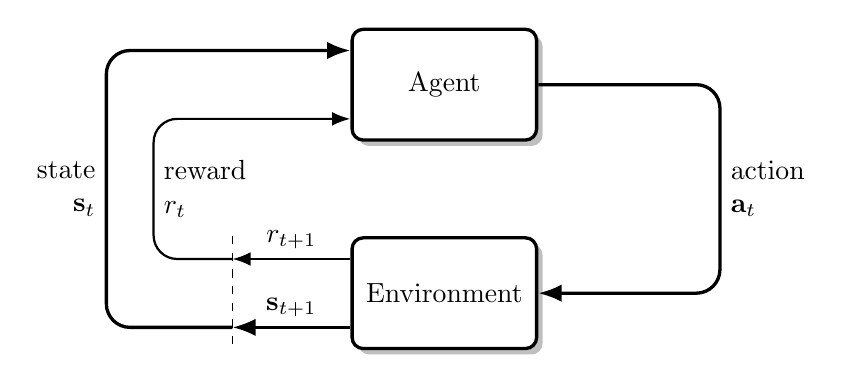
\begin{tikzpicture}[very thick,node distance = 4cm]
			\node [frame] (agent) {Agent};
			\node [frame, below=1.2cm of agent] (environment) {Environment};
			\draw[line] (agent) -- ++ (3.5,0) |- (environment)
			node[right,pos=0.25,align=left] {action\\ $\vb{a}_t$};
			\coordinate[left=15mm of environment] (P);
			\draw[thin,dashed] (P|-environment.north) -- (P|-environment.south);
			\draw[line] (environment.200) -- (P |- environment.200)
			node[midway,above]{$\vb{s}_{t+1}$};
			\draw[line,thick] (environment.160) -- (P |- environment.160)
			node[midway,above]{$r_{t+1}$};
			\draw[line] (P |- environment.200) -- ++ (-1.6,0) |- (agent.160)
			node[left, pos=0.25, align=right] {state\\ $\vb{s}_t$};
			\draw[line,thick] (P |- environment.160) -- ++ (-1,0) |- (agent.200)
			node[right,pos=0.25,align=left] {reward\\ $r_t$};
		\end{tikzpicture}}
	\end{center}
	\caption{The agent-environment process in a Markov decision process~\cite{Sutton}.}
	\label{fig:agent_env}
\end{figure}

The agent discovers complex dynamical model that helps its decision-making without external supervision. This process is formalized as an MDP, a classical model for sequential decision-making that integrates actions with feedback. The MDP serves as the theoretical foundation for reinforcement learning, providing an idealized mathematical framework for the problem.
In the context of an infinite-horizon, discounted framework, a Markov Decision Process is mathematically characterized by the tuple \( \langle A, S, P, r, q_0, \gamma \rangle \), where \( A \) and \( S \) denote the collections of all potential actions and states, respectively. The function \( P: S \times A \times S \to [0, 1] \) 
which defines the probability of moving from one state to another as a result of taking a specific action. The reward function is denoted by \( r: S \to \mathbb{R} \), mapping states to real-valued rewards. 
The initial state distribution is represented by \( q_0 \), while \( \gamma \in [0, 1] \) is the discount factor, governing the present value of future rewards.



% The Markov property, which asserts that future states depend solely on the current state and not on the sequence of past events, must hold for a problem to be appropriately modeled as an MDP. In many real-world applications, the agent receives only partial environmental data, with incomplete information available. This incomplete data is termed an observation, which parallels the state signal. Systems with such partial information are referred to as Partially Observable Markov Decision Processes (POMDPs). In POMDPs, the distinction between state and observation is crucial, as it underscores the agent's reliance on limited information. However, in this study, which assumes a fully observable MDP, this distinction is not relevant, as the observation \( o_t \) is treated as equivalent to the state \( s_t \) for simplicity.

By weighing both present and future returns, an agent aims to create a policy that maximizes its anticipated rewards and \( G_t \), expected return, is defined as the sum of future discounted benefits, which is how this balance is formalized:
\begin{align}
    G_t = \sum_{k=t+1}^{T} \gamma^{k-t-1} r_k,
\end{align}
where \( \gamma\) determines the relative importance of the present and future rewards.
All future benefits are seen as equally significant when \( \gamma = 1 \), whereas just the present reward is taken into consideration when \( \gamma = 0 \).
The value function tells the agent about the quality of a specific state, is formalized as a result of the notion of expected return.
For an MDP, the state-value function \( V^\pi(s_t) \) is described as
\begin{equation}
	V^\pi(s_t) = \mathbb{E}_\pi \left[ G_t | s_t \right] = \mathbb{E}_\pi \left[ \sum_{k=t+1}^{T} \gamma^{k-t-1} r_k | s_t \right],
\end{equation}
where \( \pi \) denotes the policy that the agent follows. The action-value function \( Q^\pi(s_t, a_t) \) is described as
\begin{equation}
	Q^\pi(s_t, a_t) = \mathbb{E}_\pi \left[ G_t | s_t, a_t \right] = \mathbb{E}_\pi \left[ \sum_{k=t+1}^{T} \gamma^{k-t-1} r_k | s_t, a_t \right],
\end{equation}
which represents the expected return when the agent is in state \( s_t \), takes action \( a_t \), and follows policy \( \pi \) thereafter. The value functions and action-value functions are related by
\begin{equation}
	V^\pi(s_t) = \mathbb{E}_{a_t \sim \pi} \left[ Q^\pi(s_t, a_t) \right].
\end{equation}
Policy optimization techniques aim to directly derive a parameterized control policy, \( \pi_\theta(a | s) \), where \( \theta \) denotes the policy parameters.
 Unlike methods using value optimization, like Deep Q-Networks (DQN) and \( Q \)-Learning, policy optimization is particularly effective for problems with continuous action spaces.
%   In complex control tasks, where discretization may impose limitations, the ability to handle both continuous state and action spaces provides a significant advantage and enhances scalability to higher-dimensional dynamical models.

A prominent class of reinforcement learning methods consists of hybrid algorithms, commonly referred to as actor-critic frameworks. These approaches simultaneously optimize the policy (the actor) and the value function (the critic), with both components use neural networks. Among various actor-critic schemes, Deep Deterministic Policy Gradient (DDPG)~\cite{DDPG} is particularly suited for continuous action spaces and is employed in this study. DDPG has demonstrated considerable success in high-dimensional continuous control tasks and is the method of choice for this investigation.


\subsubsection{Neural Networks}
Neural networks are a category of machine learning architectures that are inspired by the human brain. 
Neural networks are composed of interconnected units, commonly referred to as neurons, arranged in hierarchical layers. Each neuron receives input from the preceding layer, applies a nonlinear activation function, and generates an output that is forwarded to the subsequent layer. These networks possess the capability to model intricate patterns and dependencies within data, enabling them to excel in a diverse array of machine learning applications, including image classification, natural language processing, and reinforcement learning.



\subsection{Deep Deterministic Policy Gradient Differential Game}
The Deep Deterministic Policy Gradient Differential Game (DDPG-DG) approach combines the strengths of reinforcement learning with differential game theory to address control challenges in multi-agent, continuous action settings. By leveraging the DDPG algorithm within a differential game framework, this method enables the simultaneous optimization of policies for interacting agents, providing a robust solution to complex, real-world dynamic control problems. The following section details the formulation and implementation of DDPG-DG for spacecraft guidance in multi-body environments.


\subsubsection{Policy and Value Functions}

In the context of the Deep Deterministic Policy Gradient Differential Game (DDPG-DG), the system involves two agents, each of which learns a deterministic policy \( \pi_{\theta}(s) \) that maps states \( s \) to actions \( a \). These policies are parameterized by neural networks with weights \( \theta \), and the objective is to optimize the policy parameters to maximize the expected cumulative return. For simplicity and clarity, the same notation \( \pi \) used for the policies of both agents, as their policies follow the same functional form and differ only in their individual parameters.

The action-value function (Q-function) is defined as the expected return of taking action \( a \) in state \( s \), following the policy \( \pi \). The Q-function is given by:
\begin{equation}
    Q^{\pi}(s, a) = \mathbb{E} \left[ \sum_{t=0}^{T} \gamma^t r_t | s_0 = s, a_0 = a, \pi \right],
\end{equation}
where \( r_t \) denotes the reward received at time step \( t \), and \( \gamma \in [0, 1] \) is the discount factor. The goal of DDPG is to learn the optimal action-value function, \( Q^{\pi^*}(s, a) \), which provides the expected return for each state-action pair under the optimal policy.
% add actor and critic networks
The actor network \( \pi_{\theta}(s) \) is responsible for selecting actions, while the critic network \( Q_{\phi}(s, a) \) evaluates these actions by computing the Q-value. The actor network outputs the action directly, while the critic network estimates the Q-value for a given state-action pair. Both networks are trained using the DDPG algorithm to optimize the policy and value functions.
The structure of the actor and critic networks is shown in Fig.~\ref{fig:actor_nn} and Fig.~\ref{fig:critic_nn}, respectively. The actor network and critic network consist of fully connected layers with ReLU activation functions. The actor network outputs the action directly, while the critic network estimates the Q-value for a given state-action pair. The actor network is trained to maximize the Q-value, while the critic network is trained to minimize the error between the predicted Q-value and the target Q-value.
% NEURAL NETWORKS
\begin{figure}[H]
	\centering
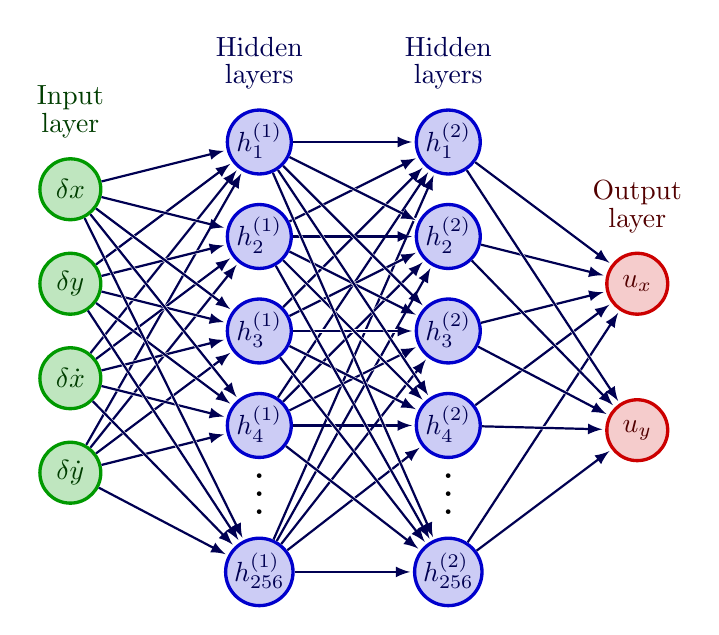
\begin{tikzpicture}[x=2.4cm,y=1.2cm]
	\readlist\Nnod{4,5,5,2} % array of number of nodes per layer
	\readlist\Nstr{n,256,k} % array of string number of nodes per layer
	\readlist\Cstr{x,h^{(\prev)},u} % array of coefficient symbol per layer
	\def\yshift{0.55} % shift last node for dots
	
	% LOOP over LAYERS
% LOOP over LAYERS
\foreachitem \N \in \Nnod{
  \def\lay{\Ncnt} % alias of index of current layer
  \pgfmathsetmacro\prev{int(\Ncnt-1)} % number of previous layer
  \foreach \i [evaluate={\c=int(\i==\N); 
  \layercheck=\ifnum\Ncnt=1 0 \else \ifnum\Ncnt=\Nnodlen 0 \else \yshift \fi \fi;
  \y=\N/2-\i-\c*\layercheck;
  \x=\lay; \n=\nstyle;
  \index=(\i<\N?int(\i):"\Nstr[\n]");}] in {1,...,\N}{ % loop over nodes
    % NODES
	\ifnum \lay=1
	\ifnum \i=1
		\node[node \n] (N\lay-\i) at (\x,\y) {$\delta x$};
	\fi
	\ifnum \i=2
		\node[node \n] (N\lay-\i) at (\x,\y) {$\delta y$};
	\fi
	\ifnum \i=3
		\node[node \n] (N\lay-\i) at (\x,\y) {$\delta {\dot{x}}$};
	\fi
	\ifnum \i=4
		\node[node \n] (N\lay-\i) at (\x,\y) {$\delta {\dot{y}}$};
	\fi
	\else \ifnum \lay=\Nnodlen
	\ifnum \i=1
		\node[node \n] (N\lay-\i) at (\x,\y) {$u_x$};
	\fi
	\ifnum \i=2
		\node[node \n] (N\lay-\i) at (\x,\y) {$u_y$};
	\fi
	\else
    \node[node \n] (N\lay-\i) at (\x,\y) {$\strut\Cstr[\n]_{\index}$};
    \fi \fi
    % CONNECTIONS
    \ifnumcomp{\lay}{>}{1}{ % connect to previous layer
      \foreach \j in {1,...,\Nnod[\prev]}{ % loop over nodes in previous layer
        \draw[white,line width=1.2,shorten >=1] (N\prev-\j) -- (N\lay-\i);
        \draw[connect] (N\prev-\j) -- (N\lay-\i);
      }
    %   \ifnum \lay=\Nnodlen
    %     \draw[connect] (N\lay-\i) --++ (0.5,0); % arrows out
    %   \fi
    }{
    %   \draw[connect] (0.5,\y) -- (N\lay-\i); % arrows in
    }
  }

  % Dots (skip first and last layers)
  \ifnum \lay>1 \ifnum \lay<\Nnodlen
    \path (N\lay-\N) --++ (0,1+\yshift) node[midway,scale=1.6] {$\vdots$}; % dots
  \fi \fi
}

  
	
	% LABELS
	\node[above=.1,align=center,mydarkgreen] at (N1-1.90) {Input\\[-0.2em]layer};
	\node[above=.1,align=center,mydarkblue] at (N2-1.90) {Hidden\\[-0.2em]layers};
	\node[above=.1,align=center,mydarkblue] at (N3-1.90) {Hidden\\[-0.2em]layers};
	\node[above=.1,align=center,mydarkred] at (N\Nnodlen-1.90) {Output\\[-0.2em]layer};
  \end{tikzpicture}
  \caption{Neural network architecture of the actor in the DDPG algorithm.}
\end{figure}
\begin{figure}[H]
	\centering
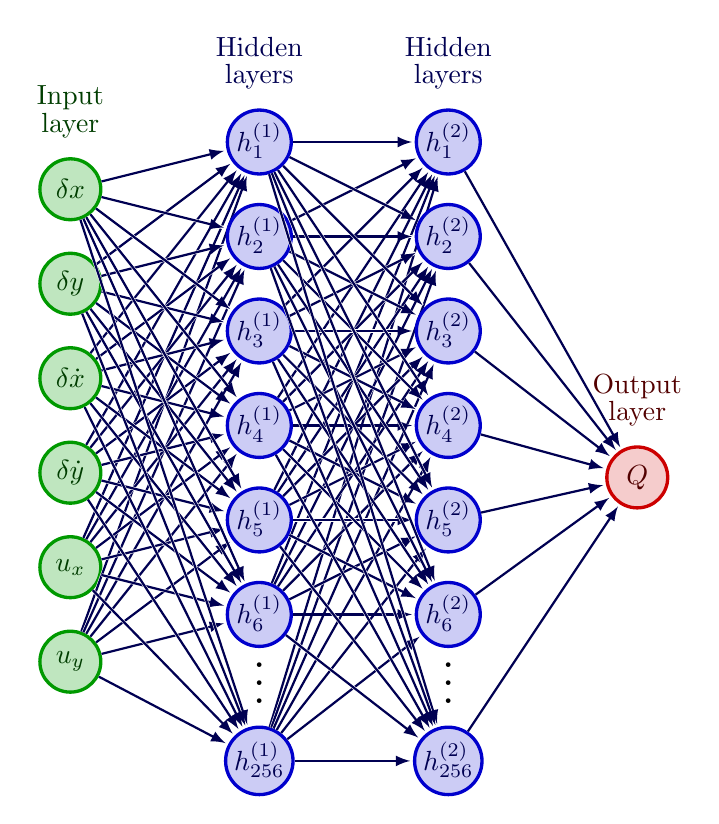
\begin{tikzpicture}[x=2.4cm,y=1.2cm]
	\readlist\Nnod{6,7,7,1} % array of number of nodes per layer
	\readlist\Nstr{n,256,k} % array of string number of nodes per layer
	\readlist\Cstr{x,h^{(\prev)},u} % array of coefficient symbol per layer
	\def\yshift{0.55} % shift last node for dots
	
	% LOOP over LAYERS
% LOOP over LAYERS
\foreachitem \N \in \Nnod{
  \def\lay{\Ncnt} % alias of index of current layer
  \pgfmathsetmacro\prev{int(\Ncnt-1)} % number of previous layer
  \foreach \i [evaluate={\c=int(\i==\N); 
  \layercheck=\ifnum\Ncnt=1 0 \else \ifnum\Ncnt=\Nnodlen 0 \else \yshift \fi \fi;
  \y=\N/2-\i-\c*\layercheck;
  \x=\lay; \n=\nstyle;
  \index=(\i<\N?int(\i):"\Nstr[\n]");}] in {1,...,\N}{ % loop over nodes
    % NODES
	\ifnum \lay=1
	\ifnum \i=1
		\node[node \n] (N\lay-\i) at (\x,\y) {$\delta x$};
	\fi
	\ifnum \i=2
		\node[node \n] (N\lay-\i) at (\x,\y) {$\delta y$};
	\fi
	\ifnum \i=3
		\node[node \n] (N\lay-\i) at (\x,\y) {$\delta {\dot{x}}$};
	\fi
	\ifnum \i=4
		\node[node \n] (N\lay-\i) at (\x,\y) {$\delta {\dot{y}}$};
	\fi
    \ifnum \i=5
        \node[node \n] (N\lay-\i) at (\x,\y) {$u_x$};
    \fi
    \ifnum \i=6
        \node[node \n] (N\lay-\i) at (\x,\y) {$u_y$};
    \fi
	\else \ifnum \lay=\Nnodlen
	\ifnum \i=1
		\node[node \n] (N\lay-\i) at (\x,\y) {$Q$};
	\fi
	\ifnum \i=2
		\node[node \n] (N\lay-\i) at (\x,\y) {$u_y$};
	\fi
	\else
    \node[node \n] (N\lay-\i) at (\x,\y) {$\strut\Cstr[\n]_{\index}$};
    \fi \fi
    % CONNECTIONS
    \ifnumcomp{\lay}{>}{1}{ % connect to previous layer
      \foreach \j in {1,...,\Nnod[\prev]}{ % loop over nodes in previous layer
        \draw[white,line width=1.2,shorten >=1] (N\prev-\j) -- (N\lay-\i);
        \draw[connect] (N\prev-\j) -- (N\lay-\i);
      }
    %   \ifnum \lay=\Nnodlen
    %     \draw[connect] (N\lay-\i) --++ (0.5,0); % arrows out
    %   \fi
    }{
    %   \draw[connect] (0.5,\y) -- (N\lay-\i); % arrows in
    }
  }

  % Dots (skip first and last layers)
  \ifnum \lay>1 \ifnum \lay<\Nnodlen
    \path (N\lay-\N) --++ (0,1+\yshift) node[midway,scale=1.6] {$\vdots$}; % dots
  \fi \fi
}

  
	
	% LABELS
	\node[above=.1,align=center,mydarkgreen] at (N1-1.90) {Input\\[-0.2em]layer};
	\node[above=.1,align=center,mydarkblue] at (N2-1.90) {Hidden\\[-0.2em]layers};
	\node[above=.1,align=center,mydarkblue] at (N3-1.90) {Hidden\\[-0.2em]layers};
	\node[above=.1,align=center,mydarkred] at (N\Nnodlen-1.90) {Output\\[-0.2em]layer};
  \end{tikzpicture}
  \caption{Neural network architecture of the critic in the DDPG algorithm.}
\end{figure}
\subsubsection{DDPG-DG Objective}

The DDPG algorithm involves optimizing two primary functions: the policy function (actor) and the Q-function (critic). The actor is responsible for selecting actions, while the critic evaluates these actions by computing the Q-value.

The policy gradient is given by the deterministic policy gradient theorem, which states that the gradient of the expected return with respect to the policy parameters can be expressed as:

\begin{equation}
    \nabla_{\theta} J(\theta) = \mathbb{E} \left[ \nabla_{\theta} \pi_{\theta}(s) \nabla_a Q(s, a) |_{a = \pi_{\theta}(s)} \right],
\end{equation}
where \( \nabla_{\theta} \pi_{\theta}(s) \) is the gradient of the policy with respect to its parameters, and \( \nabla_a Q(s, a) \) is the gradient of the Q-function with respect to the action.

For the Q-function, the update rule is based on the Bellman equation for continuous action spaces, which provides a target for the Q-function update. The Bellman backup equation is given by:

\begin{equation}
    y = r + \gamma Q'(s', a'; \theta^-),
\end{equation}
where \( r \) is the immediate reward, \( s' \) is the next state, \( a' \) is the action chosen by the target policy \( \pi_{\theta^-}(s') \), and \( Q'(s', a'; \theta^-) \) is the target Q-value. The target Q-value is estimated using the target Q-network, which has parameters \( \theta^- \) and is periodically updated to stabilize training.

\subsubsection{DDPG-DG Algorithm}

The DDPG-DG algorithm is implemented using two neural networks: the actor network \( \pi_{\theta}(s) \) and the critic network \( Q_{\theta}(s, a) \). These networks are trained using the following algorithm:

% \begin{algorithm}[H]
%     \caption{Deep Deterministic Policy Gradient Differential
% 	Game}
%     \label{alg1}
% \begin{algorithmic}[1]
%     \STATE Input: initial policy parameters $\theta$, Q-function parameters $\phi$, empty replay buffer $\mathcal{D}$
%     \STATE Set target parameters equal to main parameters $\theta_{\text{targ}} \leftarrow \theta$, $\phi_{\text{targ}} \leftarrow \phi$
%     \REPEAT
%         \STATE Observe state $s$ and select action $a = \text{clip}(\mu_{\theta}(s) + \epsilon, a_{Low}, a_{High})$, where $\epsilon \sim \mathcal{N}$
%         \STATE Execute $a$ in the environment
%         \STATE Observe next state $s'$, reward $r$, and done signal $d$ to indicate whether $s'$ is terminal
%         \STATE Store $(s,a,r,s',d)$ in replay buffer $\mathcal{D}$
%         \STATE If $s'$ is terminal, reset environment state.
%         \IF{it's time to update}
%             \FOR{however many updates}
%                 \STATE Randomly sample a batch of transitions, $B = \{ (s,a,r,s',d) \}$ from $\mathcal{D}$
%                 \STATE Compute targets
%                 \begin{equation*}
%                     y(r,s',d) = r + \gamma (1-d) Q_{\phi_{\text{targ}}}(s', \mu_{\theta_{\text{targ}}}(s'))
%                 \end{equation*}
%                 \STATE Update Q-function by one step of gradient descent using
%                 \begin{equation*}
%                     \nabla_{\phi} \frac{1}{|B|}\sum_{(s,a,r,s',d) \in B} \left( Q_{\phi}(s,a) - y(r,s',d) \right)^2
%                 \end{equation*}
%                 \STATE Update policy by one step of gradient ascent using
%                 \begin{equation*}
%                     \nabla_{\theta} \frac{1}{|B|}\sum_{s \in B}Q_{\phi}(s, \mu_{\theta}(s))
%                 \end{equation*}
%                 \STATE Update target networks with
%                 \begin{align*}
%                     \phi_{\text{targ}} &\leftarrow \rho \phi_{\text{targ}} + (1-\rho) \phi \\
%                     \theta_{\text{targ}} &\leftarrow \rho \theta_{\text{targ}} + (1-\rho) \theta
%                 \end{align*}
%             \ENDFOR
%         \ENDIF
%     \UNTIL{convergence}
% \end{algorithmic}
% \end{algorithm}



\begin{algorithm}[H]
    \caption{Deep Deterministic Policy Gradient Differential Game}
    \label{alg1}
\begin{algorithmic}[1]
    \STATE Input: initial policy parameters $\theta_1$, $\theta_2$, Q-function parameters $\phi_1$, $\phi_2$, empty replay buffer $\mathcal{D}$
    \STATE Set target parameters equal to main parameters $\theta_{\text{targ},1} \leftarrow \theta_1$, $\theta_{\text{targ},2} \leftarrow \theta_2$, $\phi_{\text{targ},1} \leftarrow \phi_1$, $\phi_{\text{targ},2} \leftarrow \phi_2$
    \REPEAT
        \STATE Observe state $s$ and select actions for both players $a_1 = \text{clip}(\mu_{\theta_1}(s) + \epsilon_1, a_{Low}, a_{High})$ and $a_2 = \text{clip}(\mu_{\theta_2}(s) + \epsilon_2, a_{Low}, a_{High})$, where $\epsilon_1 \sim \mathcal{N}$ and $\epsilon_2 \sim \mathcal{N}$
        \STATE Execute actions $(a_1, a_2)$ in the environment
        \STATE Observe next state $s'$, reward pair $(r_1, r_2)$ for both players, and done signal $d$
        \STATE Store $(s, a_1, a_2, r_1, r_2, s', d)$ in replay buffer $\mathcal{D}$
        \STATE If $s'$ is terminal, reset environment state.
        \IF{it's time to update}
            \FOR{however many updates}
                \STATE Randomly sample a batch of transitions, $B = \{ (s, a_1, a_2, r_1, r_2, s', d) \}$ from $\mathcal{D}$

                \STATE Compute targets for both players:
                \begin{equation*}
                    y_1 = r_1 + \gamma (1 - d) Q_{\phi_{\text{targ},1}}(s', \mu_{\theta_{\text{targ},1}}(s'), \mu_{\theta_{\text{targ},2}}(s'))
                \end{equation*}
                \begin{equation*}
                    y_2 = r_2 + \gamma (1 - d) Q_{\phi_{\text{targ},2}}(s', \mu_{\theta_{\text{targ},1}}(s'), \mu_{\theta_{\text{targ},2}}(s'))
                \end{equation*}

                \STATE Update Q-functions for both players by one step of gradient descent:
                \begin{equation*}
                    \nabla_{\phi_1} \frac{1}{|B|} \sum_{B} \left( Q_{\phi_1}(s, a_1, a_2) - y_1(r_1, s', d) \right)^2
                \end{equation*}
                \begin{equation*}
                    \nabla_{\phi_2} \frac{1}{|B|} \sum_{B} \left( Q_{\phi_2}(s, a_1, a_2) - y_2(r_2, s', d) \right)^2
                \end{equation*}

                \STATE Update policies for both players by one step of gradient ascent:
                \begin{equation*}
                    \nabla_{\theta_1} \frac{1}{|B|} \sum_{s \in B} Q_{\phi_1}(s, \mu_{\theta_1}(s), \mu_{\theta_2}(s))
                \end{equation*}
                \begin{equation*}
                    \nabla_{\theta_2} \frac{1}{|B|} \sum_{s \in B} Q_{\phi_2}(s, \mu_{\theta_1}(s), \mu_{\theta_2}(s))
                \end{equation*}

                \STATE Update target networks for both players:
                \begin{align*}
                    \phi_{\text{targ},1} &\leftarrow \rho \phi_{\text{targ},1} + (1 - \rho) \phi_1 \\
                    \phi_{\text{targ},2} &\leftarrow \rho \phi_{\text{targ},2} + (1 - \rho) \phi_2 \\
                    \theta_{\text{targ},1} &\leftarrow \rho \theta_{\text{targ},1} + (1 - \rho) \theta_1 \\
                    \theta_{\text{targ},2} &\leftarrow \rho \theta_{\text{targ},2} + (1 - \rho) \theta_2
                \end{align*}
            \ENDFOR
        \ENDIF
    \UNTIL{convergence}
\end{algorithmic}
\end{algorithm}





\subsection{Exploration and Exploitation}
In DDPG-DG, the exploration of the environment is achieved by adding noise to the action selection process. This noise, typically Gaussian or Ornstein-Uhlenbeck noise, encourages the agent to explore the environment while still utilizing the learned policy. The balance between exploration and exploitation is maintained throughout the training process, with the noise gradually decaying as the policy converges.






\subsection{Environment Configuration}
The environment for the differential game-based guidance strategy is designed to capture the dynamics of the Circular Restricted Three-Body Problem (CR3BP) with low-thrust terms. The CR3BP is a classical dynamical system that models the motion of a spacecraft in the vicinity of two primary bodies, such as the Earth and the Moon, where the gravitational forces of the two bodies dominate the spacecraft's motion. The low-thrust terms represent the effects of a continuous thrust engine on the spacecraft's trajectory, allowing for more precise control over the spacecraft's motion.
\subsubsection{State Representation}
The state of the environment is defined by the position and velocity vectors of the spacecraft in the rotating frame of the CR3BP. The state vector is given by \( \boldsymbol{s} = \begin{bmatrix}
	\delta x & \delta y & \delta \dot{x} & \delta \dot{y}
\end{bmatrix}^\mathrm{T} \), where \( \delta x \) and \( \delta y \) are the deviations in the spacecraft's position from the nominal trajectory, and \( \delta \dot{x} \) and \( \delta \dot{y} \) are the deviations in the spacecraft's velocity. The state vector captures the relative position and velocity of the spacecraft with respect to the nominal trajectory, providing the necessary information for the guidance strategy to make decisions.
\subsubsection{Action Representation}
The action space of the environment corresponds to the control inputs of the spacecraft, which are the thrust components along the spacecraft's body-fixed axes. The action vector is given by \( \boldsymbol{a} = \begin{bmatrix}
	u_x & u_y
\end{bmatrix}^\mathrm{T} \), where \( u_x \) and \( u_y \) represent the thrust components along the spacecraft's body-fixed axes. The action space allows the guidance strategy to adjust the thrust direction and magnitude to control the spacecraft's trajectory.
\subsubsection{Reward Function}
The reward function of the environment is designed to incentivize the spacecraft to reach the desired Lyapunov orbit while minimizing deviations from the nominal trajectory. The reward function is defined as:
\begin{equation}
	r = -\alpha \left( \delta x^2 + \delta y^2 \right) - \beta \left( \delta \dot{x}^2 + \delta \dot{y}^2 \right),
\end{equation}
where \( \alpha \) and \( \beta \) are weighting factors that determine the importance of position and velocity deviations in the reward calculation. The reward function encourages the spacecraft to reduce its position and velocity deviations, leading to a more accurate trajectory following.
% \subsection{Episode Design}
% The guidance strategy operates over multiple episodes, where each episode represents a complete transfer between Lyapunov orbits in the Earth-Moon system. The episode design includes the following key components:
% \begin{itemize}
% 	\item \textbf{Initialization
	% \item
\section{Mission Application: Libration Point Transfer}
The proposed guidance framework is applied to a mission scenario involving a transfer between Lyapunov orbits in the Earth-Moon system. The mission objective is to transfer a spacecraft from a lower-energy Lyapunov orbit to a higher-energy Lyapunov orbit using low-thrust propulsion. The guidance strategy is trained using the differential game-based reinforcement learning approach and is evaluated on its ability to perform the transfer accurately and efficiently. The mission application demonstrates the effectiveness of the guidance strategy in handling complex trajectory optimization tasks in multi-body dynamical environments.
% \subsection{Closed-Loop Controller Performance}

\subsection{Neural Network-Based Guidance}
The guidance strategy is implemented using neural networks to approximate the policy and value functions in the DDPG-DG algorithm. The actor network is responsible for selecting actions based on the current state of the environment, while the critic network evaluates the quality of these actions by estimating the Q-value. The neural networks are trained using the differential game formulation to optimize the spacecraft's trajectory during the Lyapunov orbit transfer. The guidance strategy leverages the capabilities of deep reinforcement learning to develop robust and adaptive control policies that can handle the complexities of the CR3BP dynamics and low-thrust propulsion. The results shown in Fig.~\ref{fig:trajectory} demonstrate the effectiveness of the neural network-based guidance strategy in achieving accurate and efficient trajectory optimization in the Earth-Moon system.




\begin{figure}[!h]
    \begin{tikzpicture}
        \centering
        \hspace{-20pt}
            \begin{axis}[
                % xmode=log,
                % ymode=log,
                legend style={at={(1,1)},anchor=north east
                    ,draw=none,fill=none,inner sep=2mm},
                xlabel=X, % \hertz requires SIunits
                ylabel=Y,
                % title={Trajectory of the Spacecraft},
                % grid=both,
                % minor grid style={gray!25},
                % major grid style={gray!25},
                width=1\linewidth,
                enlarge y limits=0.25,
                no marks]
                \addplot[line width=1pt,solid,color=red] %
                table[x=x,y=y,col sep=comma]{plot_data/trajectory_latex.csv};
                \addlegendentry{Trajectory}
                \addplot[line width=1pt,dashed,color=black] %
                table[x=x,y=y,col sep=comma]{plot_data/state.csv};
                \addlegendentry{DDPG-DG Trajectory}
            \end{axis}
        \end{tikzpicture}
        \caption{Trajectory of the Spacecraft}
        \label{fig:trajectory}  
\end{figure}




\section{Robustness and Generalization}
The robustness and generalization capabilities of the guidance strategy are evaluated through a series of simulation experiments that introduce disturbances, non-ideal thrust engine models, and model parameter variations. The experiments are designed to test the guidance strategy's ability to adapt to changing conditions and generalize across different mission scenarios. The results demonstrate the robustness of the guidance strategy in the presence of disturbances and model uncertainties, as well as its ability to generalize effectively across different mission scenarios and low-thrust engine models. The guidance strategy exhibits strong performance in challenging environments compared to conventional targeting guidance methods, highlighting its potential for autonomous spacecraft navigation in complex dynamical systems.
% results ploted rewards in box plot
The three scenarios considered for the robustness and generalization experiments for disturbances, non-ideal thrust engine models, and model parameter variations are shown in Fig.~\ref{fig:disturbance}, Fig.~\ref{fig:thrust}, and Fig.~\ref{fig:parameter}, respectively.

% \subsection{Generalization Across Missions}


% tikz plot
\begin{figure}[!h]
\begin{tikzpicture}
	\hspace{-10pt}
	\begin{axis}
	  [
	  ytick={1,2},
	  yticklabels={DDPG-DG, DDPG},
	  ]
	  \addplot+[
		boxplot prepared={
		  median=686.477151,
		  upper quartile=688.885704,
		  lower quartile=683.236397,
		  upper whisker=692.359664,
		  lower whisker=677.762436
		},
		] coordinates {};
	  \addplot+[
	  boxplot prepared={
		median=589.879372,
		upper quartile=690.021882,
		lower quartile=299.609773,
		upper whisker=692.640044,
		lower whisker=286.00839
	  },
	  ] coordinates {};
	\end{axis}
	% disturbance usingg 1000 samples mont carlo
  \end{tikzpicture}
  \caption{
	Comparison of the total rewards obtained by the DDPG and DDPG-DG algorithms in the presence of disturbances.
}\label{fig:disturbance}
\end{figure}







\begin{figure}[!h]
	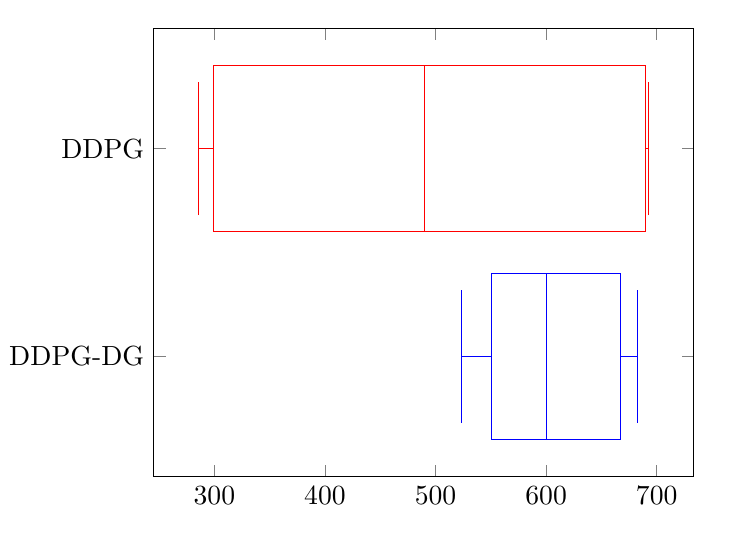
\begin{tikzpicture}
		\hspace{-10pt}
		\begin{axis}
		  [
		  ytick={1,2},
		  yticklabels={DDPG-DG, DDPG},
		  ]
		  \addplot+[
			boxplot prepared={
  lower whisker=523.236397,
  lower quartile=550.762436,
  median=600.477151,
  upper quartile=666.885704,
  upper whisker=682.359664
},
			] coordinates {};
		  \addplot+[
			boxplot prepared={
				lower whisker=286.00839,
				lower quartile=299.609773,
				median=489.879372,
				upper quartile=690.021882,
				upper whisker=692.640044
			  },
		  ] coordinates {};
		\end{axis}
		% non ideal thrust engine using 1000 samples mont carlo
	  \end{tikzpicture}
	  \caption{
		Comparison of the total rewards obtained by the DDPG and DDPG-DG algorithms in the presence of non-ideal thrust engine models.
	}\label{fig:thrust}
\end{figure}

\begin{figure}[!h]
	\begin{tikzpicture}
		\hspace{-10pt}
		\begin{axis}
		  [
		  ytick={1,2},
		  yticklabels={DDPG-DG, DDPG},
		  ]
		  \addplot+[
boxplot prepared={
	lower whisker=681.515208,
	lower quartile=683.773397,
	median=685.437301,
	upper quartile=686.945523,
	upper whisker=690.203711
  },
			] coordinates {};
		  \addplot+[
			boxplot prepared={
  lower whisker=286.00839,
  lower quartile=299.609773,
  median=689.879372,
  upper quartile=690.021882,
  upper whisker=689.640044
},
		  ] coordinates {};
		\end{axis}
		% model parameter variation 1000 samples mont carlo
	  \end{tikzpicture}
	  \caption{
		Comparison of the total rewards obtained by the DDPG and DDPG-DG algorithms in the presence of model parameter variations.
	}\label{fig:parameter}
\end{figure}










\section{Conclusion}
The proposed guidance framework leverages reinforcement learning to develop a robust differential game-based guidance strategy for low-thrust spacecraft in multi-body dynamical environments. The guidance strategy is designed to handle large initial deviations, enhance resilience against disturbances, and augment conventional targeting guidance methods. The framework is implemented using the Deep Deterministic Policy Gradient (DDPG) algorithm, which is a model-free, off-policy reinforcement learning algorithm that combines the stability of deterministic policy gradients with the flexibility of deep neural networks. The guidance strategy is trained using a differential game formulation, where two spacecraft are modeled as agents in a competitive game. The agents interact with each other and the environment to learn optimal control policies that maximize their rewards. The guidance strategy is implemented in a simulated environment that captures the dynamics of the Circular Restricted Three-Body Problem (CR3BP) with low-thrust terms. The effectiveness of the guidance strategy is demonstrated through sample transfers between Lyapunov orbits in the Earth-Moon system, where the controller exhibits strong robustness to perturbations and generalizes effectively across different mission scenarios and low-thrust engine models. The proposed guidance framework represents a significant advancement in autonomous spacecraft navigation in complex gravitational environments and has the potential to enable a wide range of deep-space missions.








% \begin{table}[htbp]
% \caption{Table Type Styles}
% \begin{center}
% \begin{tabular}{|c|c|c|c|}
% \hline
% \textbf{Table}&\multicolumn{3}{|c|}{\textbf{Table Column Head}} \\
% \cline{2-4}
% \textbf{Head} & \textbf{\textit{Table column subhead}}& \textbf{\textit{Subhead}}& \textbf{\textit{Subhead}} \\
% \hline
% copy& More table copy$^{\mathrm{a}}$& &  \\
% \hline
% \multicolumn{4}{l}{$^{\mathrm{a}}$Sample of a Table footnote.}
% \end{tabular}
% \label{tab1}
% \end{center}
% \end{table}

% \begin{figure}[htbp]
% \centerline{\includegraphics{fig1.png}}
% \caption{Example of a figure caption.}
% \label{fig}
% \end{figure}




% \section*{References}


\begin{thebibliography}{00}

\bibitem{Hart} Hart, J., King, E., Miotto, P., \& Lim, S. (n.d.). Orion GN\&C Architecture for Increased Spacecraft Automation and Autonomy Capabilities. In AIAA Guidance, Navigation and Control Conference and Exhibit. doi:10.2514/6.2008-7291
\bibitem{Clipper} Howell, S.M., Pappalardo, R.T. NASA's Europa Clipper—a mission to a potentially habitable ocean world. Nat Commun 11, 1311 (2020). https://doi.org/10.1038/s41467-020-15160-9
\bibitem{Bosanac} Bosanac, N., Cox, A. D., Howell, K. C., \& Folta, D. C. (2018). Trajectory design for a cislunar CubeSat leveraging dynamical systems techniques: The Lunar IceCube mission. Acta Astronautica, 144, 283-296. doi:10.1016/j.actaastro.2017.12.025
\bibitem{Map} Babuscia, Alessandra \& Hardgrove, Craig \& Cheung, Kar-Ming \& Scowen, Paul \& Crowell, Jim. (2017). Telecommunication system design for interplanetary CubeSat missions: LunaH-Map. 1-9. 10.1109/AERO.2017.7943826.
\bibitem{Psyche} Dibb, S. D., Asphaug, E., Bell, J. F., Binzel, R. P., Bottke, W. F., Cambioni, S., … Williams, D. A. (2024). A Post-Launch Summary of the Science of NASA's Psyche Mission. AGU Advances, 5(2), e2023AV001077. doi:10.1029/2023AV001077
\bibitem{13} Yencharis, J. D., Wiley, R. F., Davis, R. S., Holmes, Q. A., \& Zeiler, K. T. (1972). Apollo experience report: Development of guidance targeting techniques for the command module and launch vehicle (No. NASA-TN-D-6848).
\bibitem{9} B.G. Marchand, M.W. Weeks, C.W. Smith, S. Scarritt, Onboard autonomous targeting for the trans-earth phase of orion, J. Guid. Control Dyn. 33 (2010) 943-956, doi:10.2514/1.42384, https://doi.org/10.2514/1.42384.
\bibitem{11} Haapala, A. F., \& Howell, K. C. (2016). A Framework for Constructing Transfers Linking Periodic Libration Point Orbits in the Spatial Circular Restricted Three-Body Problem. International Journal of Bifurcation and Chaos, 26(05), 1630013. doi:10.1142/S0218127416300135
\bibitem{12} Marchand, B. G., Scarritt, S. K., Pavlak, T. A., \& Howell, K. C. (2013). A dynamical approach to precision entry in multi-body regimes: Dispersion manifolds. Acta Astronautica, 89, 107–120. doi:10.1016/j.actaastro.2013.02.015
\bibitem{17} Estlin, Tara \& Bornstein, Benjamin \& Gaines, Daniel \& Anderson, Robert \& Thompson, David \& Burl, Michael \& Castaño, Richard \& Judd, Michele. (2012). AEGIS automated targeting for MER opportunity rover. ACM Transactions on Intelligent Systems and Technology (TIST). 3. 10.1145/2168752.2168764.
\bibitem{18} Francis R, Estlin T, Doran G, Johnstone S, Gaines D, Verma V, Burl M, Frydenvang J, Montaño S, Wiens RC, Schaffer S, Gasnault O, DeFlores L, Blaney D, Bornstein B. AEGIS autonomous targeting for ChemCam on Mars Science Laboratory: Deployment and results of initial science team use. Sci Robot. 2017 Jun 21;2(7):eaan4582. doi: 10.1126/scirobotics.aan4582. Epub 2017 Jun 21. PMID: 33157897.
\bibitem{19} S. Higa et al., "Vision-Based Estimation of Driving Energy for Planetary Rovers Using Deep Learning and Terramechanics," in IEEE Robotics and Automation Letters, vol. 4, no. 4, pp. 3876-3883, Oct. 2019, doi: 10.1109/LRA.2019.2928765.
keywords: {Space exploration;Energy consumption;Space vehicles;Mobile robots;Deep learning;Space robotics and automation;wheeled robotics;deep learning in robotics and automation},
\bibitem{20} Rothrock, B., Kennedy, R., Cunningham, C., Papon, J., Heverly, M., \& Ono, M. (n.d.). SPOC: Deep Learning-based Terrain Classification for Mars Rover Missions. In AIAA SPACE 2016. doi:10.2514/6.2016-5539
\bibitem{DeepSpace1} Rayman, M. D., Varghese, P., Lehman, D. H., \& Livesay, L. L. (2000). Results from the Deep Space 1 technology validation mission. Acta Astronautica, 47(2), 475–487. doi:10.1016/S0094-5765(00)00087-4
\bibitem{LunarGateway} Ticker, Ronald \& Gates, Michele \& Manzella, David \& Biaggi-Labiosa, Azlin \& Lee, Ty. (2019). The Gateway Power and Propulsion Element: Setting the Foundation for Exploration and Commerce. 10.2514/6.2019-3811.
\bibitem{Sutton} Sutton, R. S., Barto, A. G. (2018 ). Reinforcement Learning: An Introduction. The MIT Press.
\bibitem{lafarge} LaFarge, N. B., Miller, D., Howell, K. C., \& Linares, R. (2021). Autonomous closed-loop guidance using reinforcement learning in a low-thrust, multi-body dynamical environment. Acta Astronautica, 186, 1-23. doi:10.1016/j.actaastro.2021.05.014
\bibitem{DDPG} Lillicrap, T. P., Hunt, J. J., Pritzel, A., Heess, N., Erez, T., Tassa, Y., … Wierstra, D. (2019). Continuous control with deep reinforcement learning. arXiv [Cs.LG]. Retrieved from http://arxiv.org/abs/1509.02971
\end{thebibliography}

% \vspace{12pt}
% \color{red}
% IEEE conference templates contain guidance text for composing and formatting conference papers. Please ensure that all template text is removed from your conference paper prior to submission to the conference. Failure to remove the template text from your paper may result in your paper not being published.

\end{document}
